\section{Methodology}
\label{sec:method}
% ========= object centric =========
Our goal is to acquire a modular based control policy for an object manipulation task from human demonstration. To this end, we take a three-step approach:
\begin{enumerate}
\item Human demonstrating a task in different contexts (Section~\ref{sec:demo}).
%\item Clustering the data to find number of modules needed in the task (subsection ~\ref{sec:cluster}).
\item Extracting human control strategies for different contexts and build multiple internal models(Section~\ref{sec:learn}).
%\item Design a controller based on the learnt multiple model  (subsection ~\ref{controller}).
\item Use the multiple models to compute motor commands for a robot(Section~\ref{sec:control}).
\end{enumerate}

Figure~\ref{fig:overview} shows an overview of our framework.

\begin{figure}
  \centering
   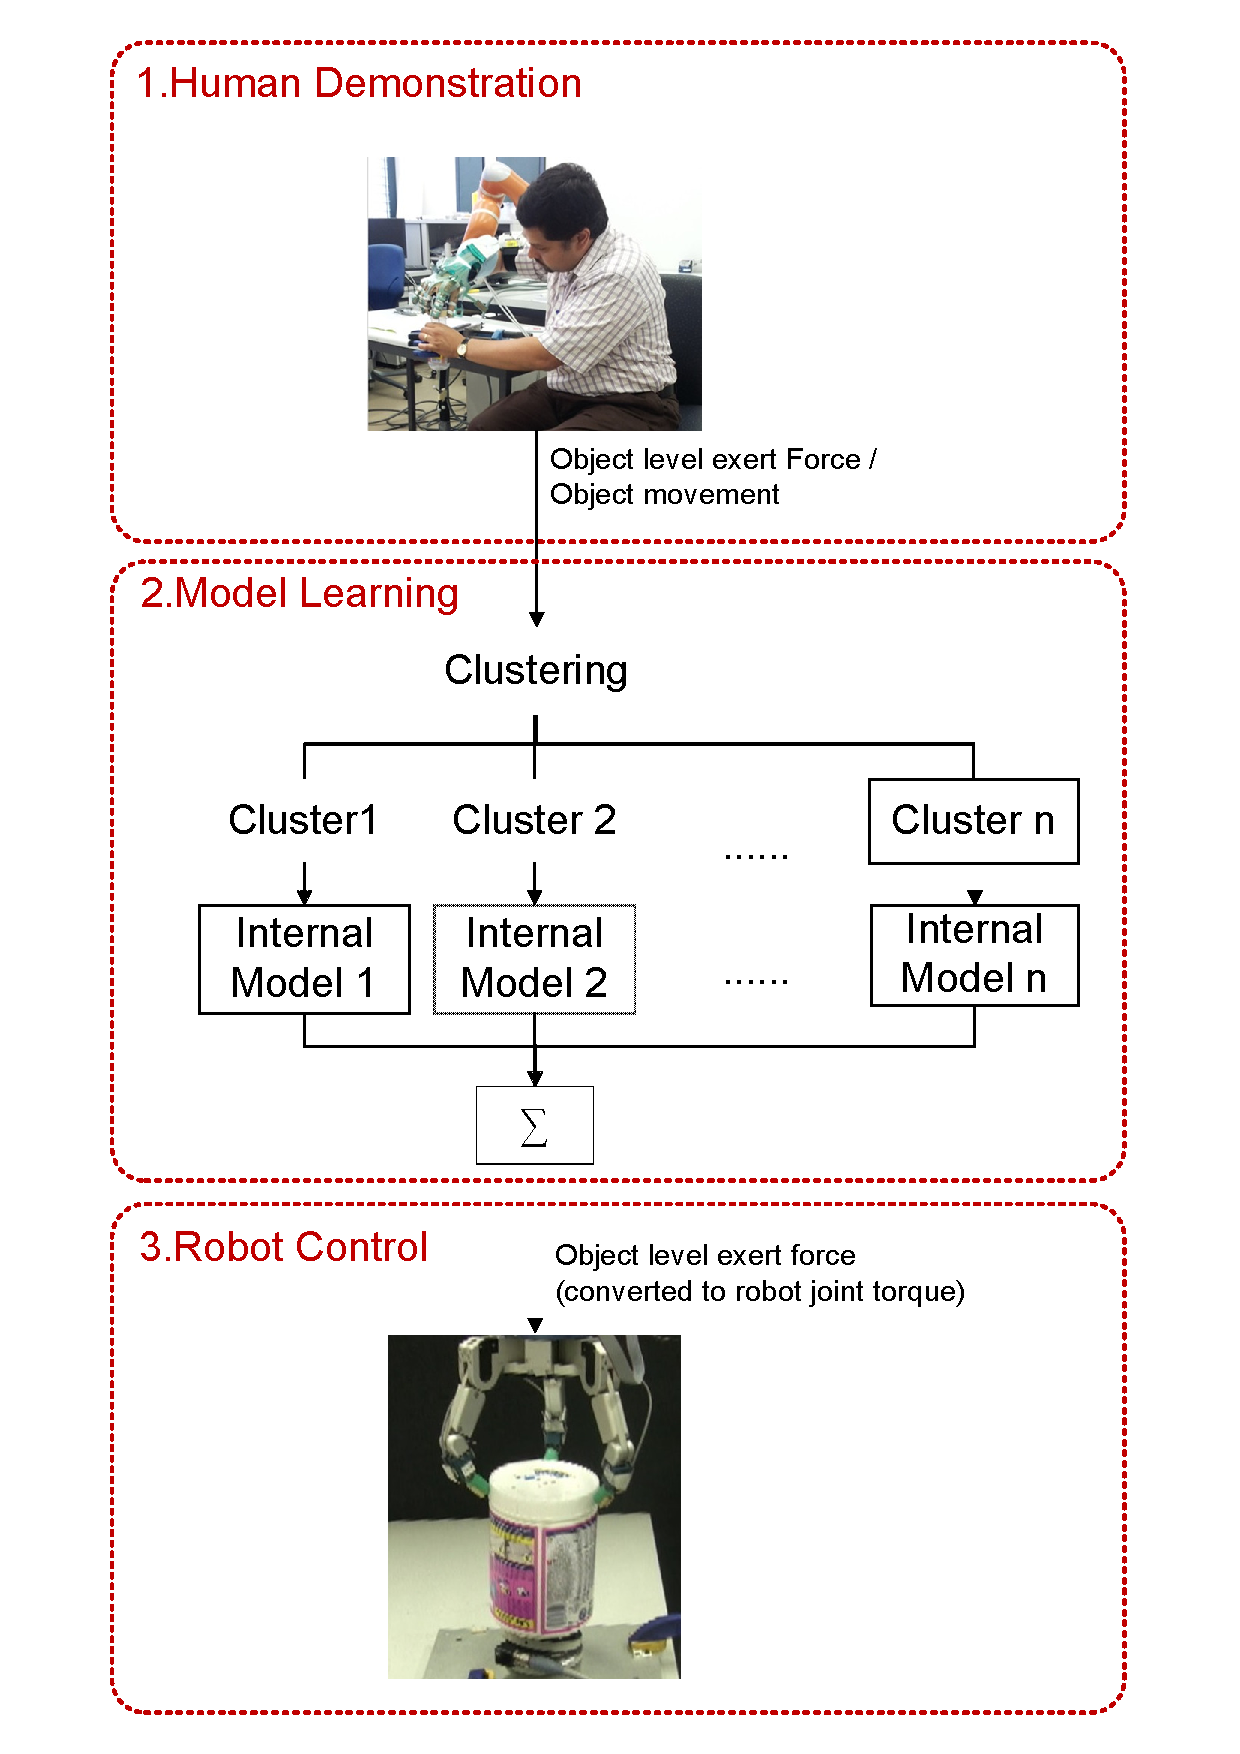
\includegraphics[width=8cm]{./fig/overview3.pdf}
  \caption{ \scriptsize{System overview.}
  \label{fig:overview}
}
\label{fig:demo}
\end{figure}

\subsection{Human demonstration}
\label{sec:demo}

%\begin{figure}
%  \centering
%   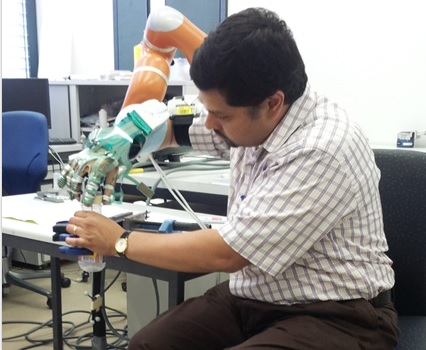
\includegraphics[width=5cm]{./fig/ravin.jpg}
%  \caption{ \scriptsize{Human demonstration of opening a bottle cap.}
%}
%\label{fig:demo}
%\end{figure}

\begin{figure}
  \centering
    \subfloat[\scriptsize{Optitrack markers attaching to a cap}] {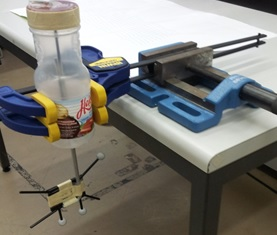
\includegraphics[height=2cm]{./fig/marker2.jpg}}
    \subfloat[\scriptsize{Force torque sensor}] {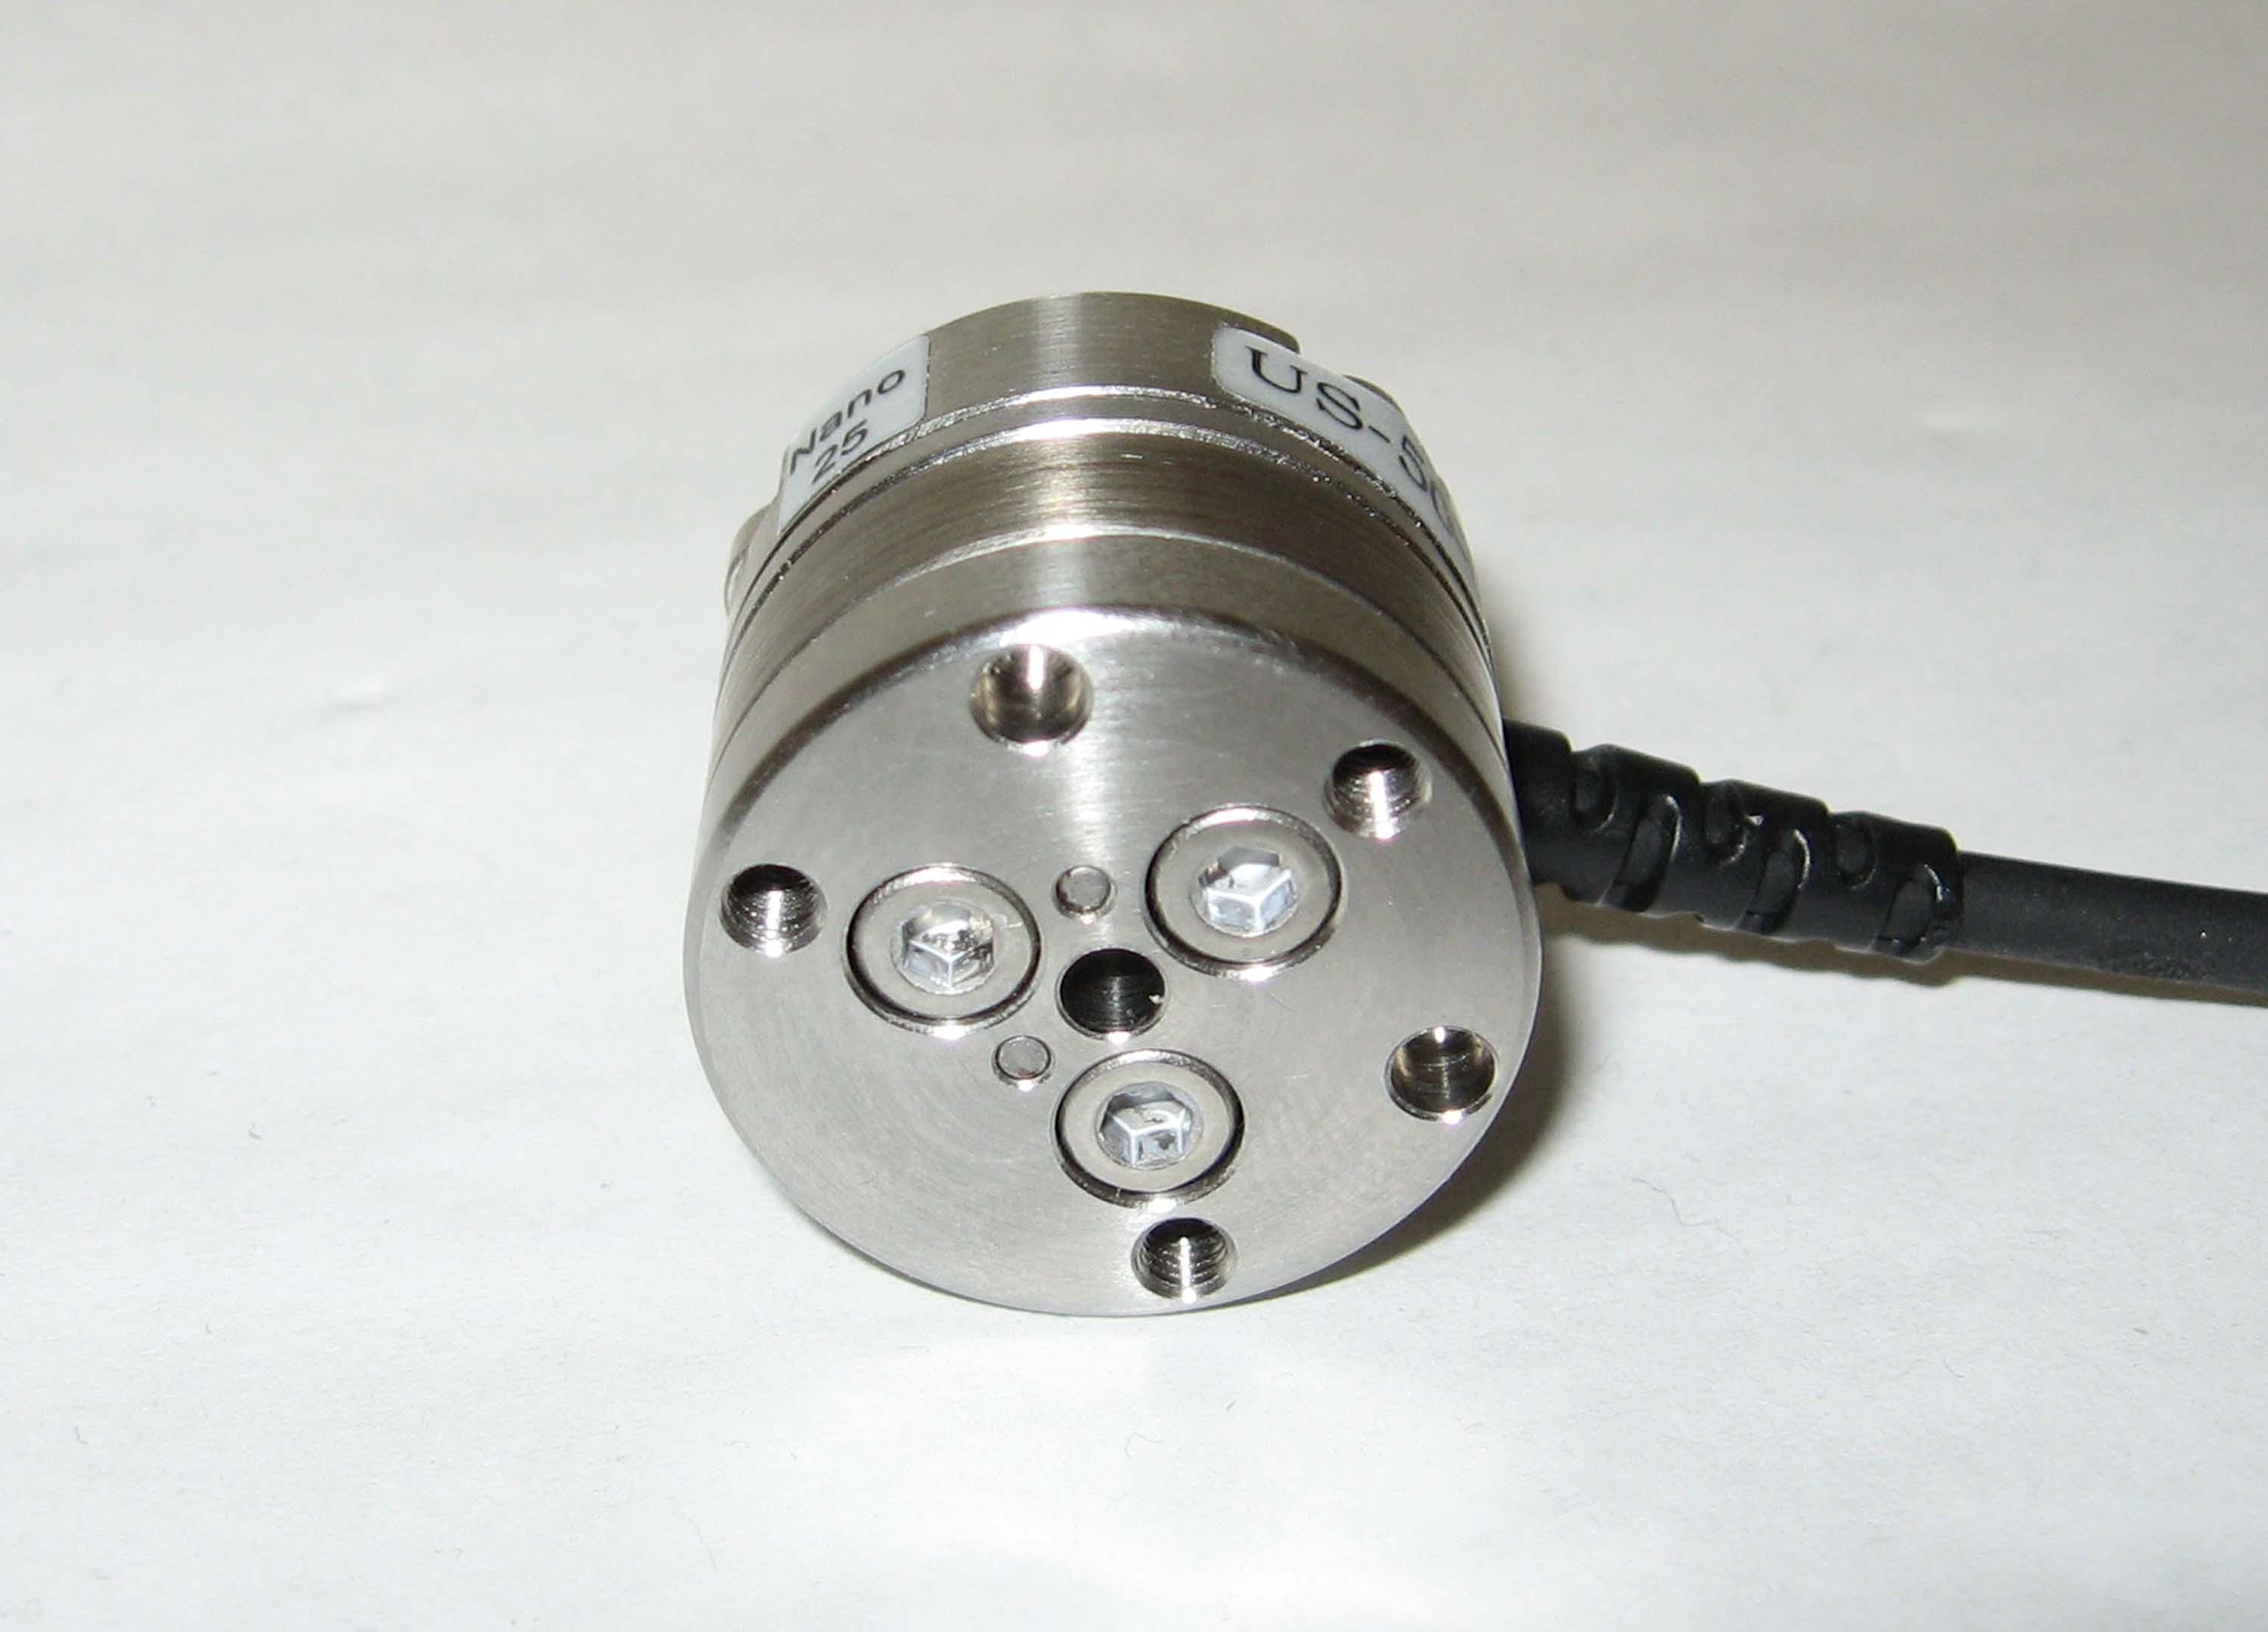
\includegraphics[height=2cm]{./fig/Nano25-E.jpg}}
    \subfloat[\scriptsize{Texscan tactile sensors mounting to a glove}] {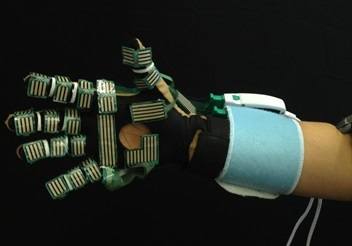
\includegraphics[height=2cm]{./fig/texscan2.jpg}}
    \caption{\scriptsize{Sensors used in the human demonstration of opening a bottle cap task.}}
  \label{fig:devices}
\end{figure}

The first step is recording human demonstration of a task. Based on the object centric principle, we collect the object trajectory and its driven force. These data can be accessed by motion capture system, force-torque sensor and wearable haptic device. Fig.~\ref{fig:devices} shows a few sensors we used in the opening bottle caps task. Details will be explained in section~\ref{sec:exp_demo}.

% ===== Why not kinematics approach? =====
%For manipulation task, kinematics teaching on robot is difficult. While a manipulation task usually involves multifinger movement, a human can kinematically operate one finger with each hand and hence two fingers simultaneously for the most extend. Tele-operation of the robot hand solves this problem but it does not provide a direct force feedback. In our approach, human perform the task with direct interaction with the object. With direct interaction with the object the teacher is able to perform the task most naturally and perform a more delicate control strategy. %In an object centric manner there is no difference between collecting data from the teacher or from the learner -- they are expressed from the objects' perspective. Once the control policy is encoded, it can be directly applied to the robots.

%Kinematics teaching of the learner is not necessary here for three reasons. Firstly in an object centric manner there is no difference between collecting data from the teacher or from the learner -- they are expressed from the object point of view. Secondly with direct interaction with the object the teacher is able to perform the task most naturally and hence provide a more naturally control policy. Thirdly manipulation with multifinger is difficult to demonstration kinematically, as a human can manipulate one finger of a robot with each hand and hence two fingers simultaneously for its most extend.

% ======= demonstrate in different context   =======
In the demonstration, the teacher perform a task a number of times to generate enough data for capturing the key features of it. Further, the teacher perform the task under different system kinematics and dynamics configurations, e.g. friction conditions, in order to explore how human adaptive to different task contexts. These different configurations are chosen to cover a wide range of different contexts. For example, in a opening bottle cap task the demonstration of opening the tightest bottle, within the capability of the learner, is included. Details will be explained in Section~\ref{sec:exp_demo}.
%How to cover ??????


%The force and torque applied on the cap are measured by the Trkscan pressure sensor and a force torque sensor. The movement of the object is recorded by the OptTrack motion tracking system. Each demonstration is recorded as a temporal sequence.

%~\cite{bidan2013robio}
%~\cite{huang2013learning}
%~\cite{huanghumanoid}
\subsection{Learning a Multiple-Module Model}
\label{sec:learn}
In this section we detail our modeling method, explaining how do we model human manipulation strategy and how to choose the number of modules of a task.

\subsubsection{Object centric manipulation strategy}
\label{sec:objectlevel}
As mentioned in Section~\ref{sec:related}, one of the challenges in imitation learning is the correspondence problem, i.e. how to map the teacher's motions to the robot's motions so that they produce the same effects, e.g. reaching the same point. %This problem is particularly important in the motion planning tasks.
In a object manipulation task, however, the goal is to deliver the object from the current state to a desired state. During this process the movement of the manipulator is bounded by the movement of the object. It is more important to imitate how human apply forces to achieve object's desired movement, than to imitate the human limb movement.
%Therefore we take an ``object centric approach"~\cite{okamura2000overview}, of which the control policy is taken from the object point of view.

Therefore, our model encodes a force and torque profile rather than the end effector movement trajectory. The imitation learning objective here is not to find a policy for the end effector movement but to find a policy that maps the force and torque to the object movement. This policy allows the robot to efficiently acquire new behaviors to accomplish the task. %Different robots move differently to achieve the desired object movements.
Giving the robots' kinematics and the desired exert force on the object, the joint torques can be deduced by the Jacobian matrix~\cite{okamura2000overview}. To this end, we focus on the force-torque-displacement tuple: $\{F,\tau,s\}$ demonstrated in the task. In later sections, we refer $\{F,\tau\}$ as the motor command with notation $\{a\}$. In each demonstration, a time series of the tuple is recorded.



\subsubsection{Decide number of modules}
\label{sec:cluster}

% ----------- why clustering -----------
Due to the involvement of object interaction, a manipulation task frequently encounter abrupt changes of the system dynamics, e.g. transfer between status of no contact to contact, of static friction and dynamic friction. Different strategies should be used to handle different dynamics. We achieve this goal by using a modular approach. Multiple modules are learned from the demonstrations under different task contexts. %During implementation, the system quickly estimate the context by the sensory inputs and choose the most appropriate module or weight and combine the modules to react.

%In this multiple model approach, each model is trained for a particular dynamics context. During the control process the model can compute appropriate control commands for the corresponding dynamics according to the sensory inputs. If the model is chosen properly (see Section~\ref{rf} for mixing model), this approach will be able to adapt to changing environmental context.

% ---------- Cluster to find number of modules -----------
Different tasks may need different number of modules. In human demonstration the same task is demonstrated with a few different setups to explore how human adapt to them. However, the number of setups does not necessary equal to the number of modules needed in the task. Human may regard different setups as the same task context and handle them with the same control strategies. %Some data may seems to be dissimilar in the scale or frequency, but in fact are governed by the same dynamic.
In order to find a proper number of modules, we need to differentiate different types of strategies. The differences can be reflected from the different pattern of the force-torque-displacement tuple. Ee differentiate the patterns in a data driven manner: cluster force-torque-displacement tuple. Data in the same cluster is considered to be governed by the same strategy. The number of clusters is the number of modules and each module is encoded by one model.


% ----------- Distance Metric for clustering ------------
The goal of clustering is to separate a set of data to a few groups according to their similarities. The first step of clustering is to measure the similarities, i.e. the distances, between different data points. Different from an usual clustering problem, the data we need to cluster are not a set of single data points but a set of time series. Here we use the Dynamic Time Warping technique (DTW) to measure the distance between each pair of time series~\cite{berndt1994using}.

Dynamic time warping is suitable for measuring the similarity between two time series, which may have different speeds or durations. It warps the data in the time dimension and finds the optimal match between the time series. The similarity is computed as the average distance between the corresponding points in two series.

The similarity (distance) between each pair of time series is computed by DTW and produce a distance matrix. In this distance matrix, each element contains a measurement of the similarity between two time series. We then cluster these time series into a few groups by a threshold of the similarity. This threshold is set by using the variance of the data from the same setup as a reference. As mentioned above, under the same setup a task is demonstrated a few times. These demonstrations are presumed to be handled with the same strategy and hence belong to the same cluster. The variance of these demonstrations give a reference of a proper variance of a cluster. The largest variance, across the variance of all setups, is used as the threshold for the clustering.

%% ------------ Hierarchical clustering -----------
Most of the clustering methods require the specification of some variables, such as the number of clusters. Without knowing the number of clusters at the first place, we use an hierarchical agglomerative clustering method~\cite{willett1988recent}. Agglomerative clustering is a method that merges data iteratively until the stop criteria satisfied, which does not require a predefined number of clusters. Our clustering method is described as follow:

\begin{enumerate}
\item At the beginning, each single time series is considered to be one cluster.
\item Compute the distances between each pair of clusters.
\item Starting from the first cluster, find its nearest cluster. We define the distance between two clusters to be the average distance across all the time series pairs in them. If the distance to the nearest cluster is smaller than the threshold, merge these two cluster.
\item Move to the next cluster. Repeat the last step for the rest of the clusters.
\item A new set of clusters are formed by the last few steps, move to the next hierarchy and repeat the step 2 to 4 until no new clusters can be formed.
\end{enumerate}

Pseudocode of the complete algorithm is shown in Algorithm~\ref{code:cluster}.

\begin{algorithm}
  \caption{Agglomerative Hierarchical Clustering}
  \begin{algorithmic}[1]
%    \Require{$x$ and $y$ are packed strings of equal length $n$}
%    \Statex Init();
    \State Init(): Make each time series a cluster\;
    \State $mergeable$ = true\;
    \Function{Merge}{all clusters, distance matrix} %      \Comment{$\oplus$: bit}
    \While{mergeable is true}
      \State $mergeable$ = false\;
      \For{each cluster}
        \State $ClusterA$ = current cluster\;
        \State $ClusterB$ = nearest neighbor of $ClusterA$\;
        \If{distance($ClusterA, ClusterB$) $<$ clustering threshold}
            \State Merge $ClusterB$ into $ClusterA$\;
            \State $mergeable$ = true\;
        \EndIf
      \EndFor
      %\State \Return{$\delta$}
    \EndWhile
    \EndFunction
  \end{algorithmic}
  \label{code:cluster}
\end{algorithm}



% --------- Number of cluster -----------
When the clusters can not be merged further, we discover the number of modules require in this task: it is the number of the remaining clusters. Each cluster is used as a module. The pattern of the data in a cluster represents a strategy of handling a specific task context.

\subsubsection{Learning Models}
\label{sec:model}
After identifying the number of modules, we build models for each of the module. In this section, we explain the way we encode human manipulation strategy.

During demonstrations, we constantly acquire the object displacements and the force and torque applied by the teacher. The teacher is the only source of exert force and torque of the system. The relationship between the exert force and torque and their resulting object displacement shows the dynamic characteristic of the task.

%GMM
In our approach, we model the correlation of the force and the displacement with GMM. The task dynamics is hence encoded as a joint distribution of the object status displacement $s$ and the action $a$ taken by human $p(s,a,{\mid}{\Omega})$. In our task, $s$ is the one dimensional cap angular displacment and $a$ is the one dimensional exert torque and grip force (section~\ref{sec:exp}).
Modeling the distribution by GMM allows us to capture the nonlinearity in the data, as well as to compute the likelihood of a query data point in the model. This provides an good estimation of the reliability of the module in the current task context, which is crucial in choosing the correct modules for control (discussed in Section~\ref{sec:rf}). At the other hand, as a generative model GMM is able to generate new data from the model, i.e. generate motor commands.

With a GMM, the joint distribution of the variables is expressed as a sum of $N$ Gaussian components,
\begin{equation}
{
p(s,a\mid\Omega)
= \sum_{n=1}^N {p_{n}p(s,a\mid{\mu}_n},{\Sigma}_n)
}
\end{equation}
where $p_n$ is the prior of the $n$-th Gaussian component and the ${\mu}_n$, ${\Sigma}_n$ the corresponding mean and covariance as:

\begin{equation}
{
{\mu}_n = \begin{pmatrix}    {\mu}_{s,n}     \\
                             {\mu}_{a,n}          \\
                    \end{pmatrix}
\hspace{0.2in}
{\Sigma}_n = \begin{pmatrix}     {\Sigma}_{ss,n}  &
                                 {\Sigma}_{sa,n} \\
                                 {\Sigma}_{as,n}  &
                                 {\Sigma}_{aa,n}   \\

                        \end{pmatrix}
}
\end{equation}

%The choice of GMM give us three advantages. Firstly, it is good in modeling nonlinear behavior. Secondly, it tolerates noisy of the data in a good extend and give good estimation of the expected values. Thirdly, as a generative model, it allows the computation of the likelihood of a given input data in the model. This provides an easy measurement of the reliability of the module, which is crucial in choosing the correct modules for control (see Section~\ref{sec:rf}).

%We use the Gaussian Mixture Model (GMM)~\cite{cohn1996active} to encode the task dynamics, and get a joint distribution of the object status $s=\{(x^t,v^t)\}^T_{t=1}$ (displacement $x$ and velocity $v$) and the action taken by human ($a=\{f^t,\tau^t\}^T_{t=1}$) $p(s, a, {\mid} {\Omega})$. The choice of GMM give us three advantages. Firstly, it is good in modeling nonlinear behaviour. Secondly, it tolerates noisy of the data in a good extend and give good estimation of the expected values. Thirdly, as a generative model it is flexible of the type of control: we can compute the force and torque from the given displacement and velocity or compute the displacement and velocity from the given force and torque. %According to different tasks, the variables encoded by GMM may be in different format, e.g. for multi-step prediction control we need to model $s$ in the form of $s=\{x^t,x^{t-1},x^{t-2},...,v^t,v^{t-1},v^{t-2},...\}$. See later section~ref{experiment} for details.


%We aim to build a model closely simulates human motor strategy in order to make the best use of the human data. Evidences of neuroscience suggest that human develop internal model for motor control, so as to estimate the outcome of a motor command. The use of internal model speed up the human correction and reaction in motor control. One hypothesis of the internal model is MOSAIC, which is a multiple modular model composed by a couple of pairs of forward model and inverse model. We build our control strategy based on this hypothesis.

%A forward model is held to anticipate the outcome of the motor command, while an inverse model is held to generate motor commands to take the current system state to the next state. The discrepancy between the anticipation of the forward model and the actual feedback is used to correct the motor command generated from the inverse model (Section~\ref{sec:rf}). Figure~\ref{fig:control} shows the basic control flow of a forward-inverse model pair.

We aim to build a model closely simulates human motor strategy in order to make the best use of the human data. A forward model is held to anticipate the outcome of the motor command, while an inverse model is held to generate motor commands to take the current system state to the next state. The discrepancy between the anticipation of the forward model and the actual feedback is used to correct the motor command generated from the inverse model (Section~\ref{sec:rf}). Figure~\ref{fig:control} shows the basic control flow of a forward-inverse model pair.

\begin{figure}
  \centering
      \subfloat[\scriptsize{}]{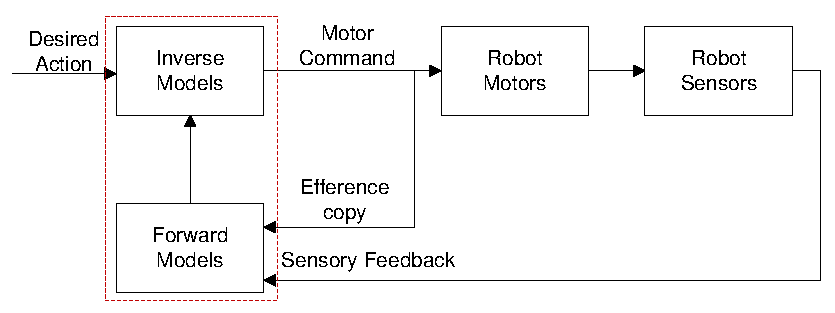
\includegraphics[width=8cm]{./fig/control_1_2.pdf}}
      \vspace{0.5cm}
      \subfloat[\scriptsize{}]{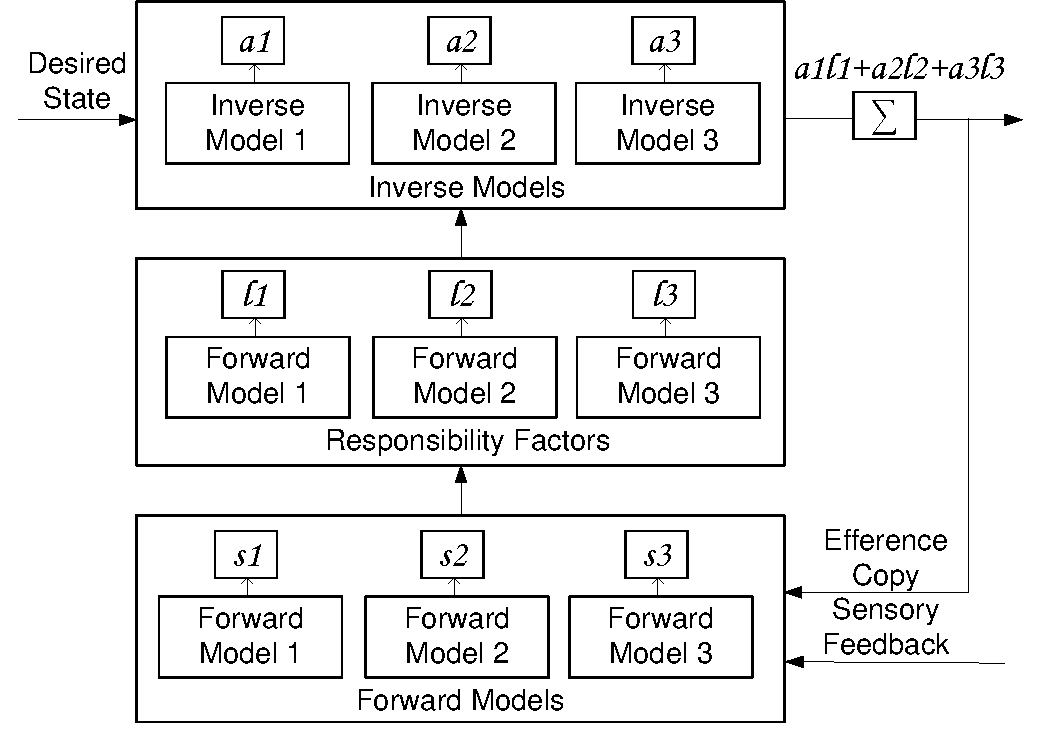
\includegraphics[width=8cm]{./fig/control_3_2.pdf}}
%  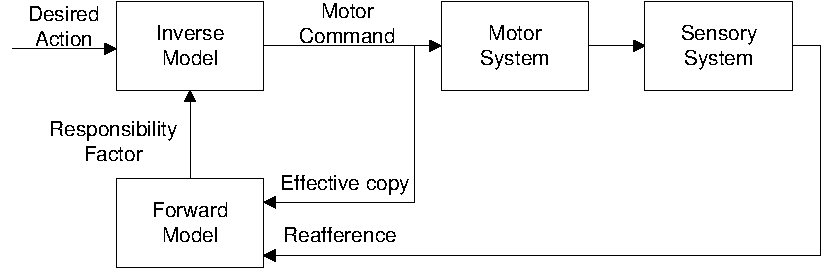
\includegraphics[width=8cm]{./fig/control_1.pdf}
%
%  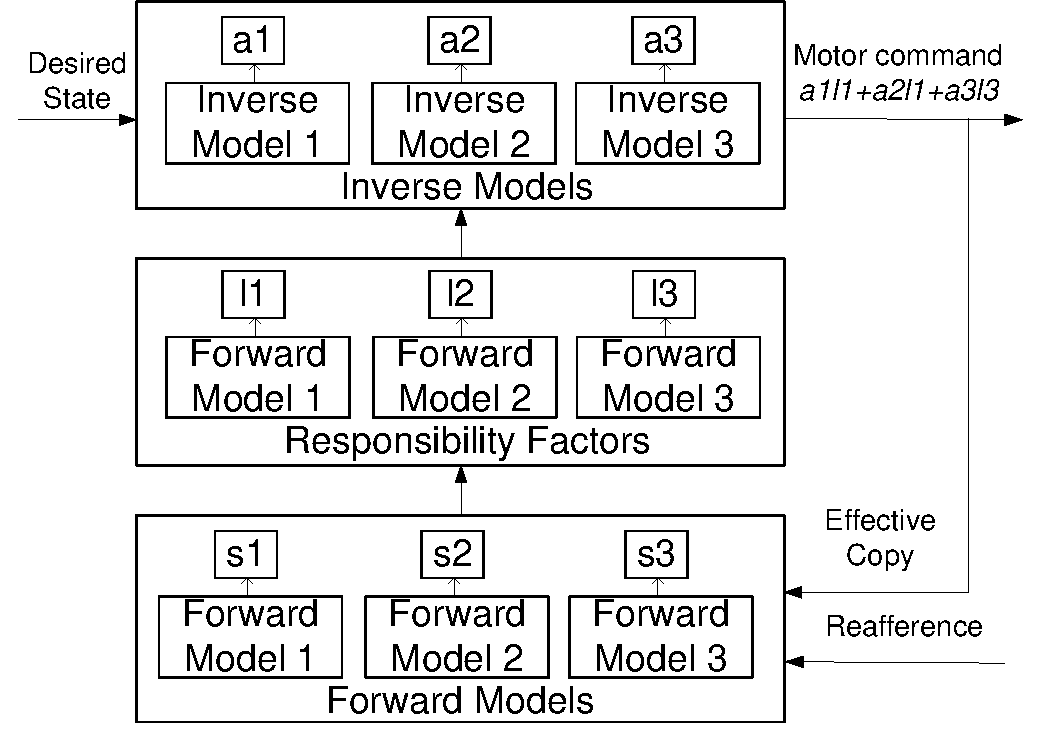
\includegraphics[width=8cm]{./fig/control_4.pdf}
  \caption{ \scriptsize{Control flow diagram of forward-inverse model in motor control. (a) System overview. Pairs of forward and inverse models work together to generate final motor command. The mechanism inside the red box is shown underneath. (b) A example of a 3 modules model. The forward models predict current task context (s1, s2, s3) and estimate the accuracy of their prediction (l1, l2, l3). These accuracy is called ``Responsibility Factors'' as they decide how much responsibility each inverse model should take in the final command. The Inverse models generate commands (a1, a2, a3) and the final command is the summation of them factorized by their responsibility factor (a1l1+a2l2+a3l3).  }
}
\label{fig:control}
\end{figure}

% ----------- One model for both -------------
%The internal model ${\Omega})$ (forward model and inverse model) is encoded by the joint distributions of the variables, i.e. $p(s_t,s_{t+1},a_{t-1},a_t\mid{\Omega})$. This joint distribution encodes the forward model and the inverse model at the same time and both of their functionalities can be realized by the Gaussian Mixture Regression (GMR). For a given previous state and previous motor command, GMR provides a close-form solution to compute the anticipating state $s_t$, i.e. $p(s_{t+1}{\mid}s_{t},a_{t},{\Omega})$. For a given current state and desired state, we can compute the motor command using GMR, i.e. $p(a_t{\mid}s_t,s^{*}_{t+1},{\Omega_f})$. In some tasks, the initial status of the system remains unchanged for a certain time until the exert force or torque is big enough to change it. This will cause degeneracy in the inverse model. To solve this problem we include the previous motor command into the model, i.e. $p(a_t{\mid}s_t,s^{*}_{t+1},a_{t-1},{\Omega_f})$.

% --------- one model for each ----------
The forward model $\Omega_I$ is encoded by the joint distributions of the current system state, previous system state and the previous motor command, i.e. $p(s_t,s_{t-1},a_{t-1}\mid{\Omega_I})$. For a given object displacement and a motor command, the Gaussian Mixture Regression (GMR) provides a close-form solution to compute the anticipating object displacement $s_t$, i.e. $E(s_t{\mid}s_{t-1},a_{t-1},{\Omega_I})$. The inverse model $\Omega_f$ is encoded by the joint distributions of the current object displacement $s_t$ and the desired object displacement $s^{*}_{t+1}$. In some tasks, the initial status of the system remains unchanged for a certain time until the exert force or torque is big enough to change it. This will cause degeneracy in the inverse model. To solve this problem we include the previous motor command into the model, i.e. $p(s_t,s^{*}_{t+1},a_{t-1},a_t{\mid}{\Omega_F})$.



% Non-linear, multi model. What to solve in multi model
%As discussed above, one of the characteristics of manipulation task is the changing kinematics and dynamics configuration.
%In different task contexts, the pattern of the correlation between the displacement and action may be different.
By clustering the training data into different groups as discussed in Section~\ref{sec:cluster}, we are able to discover the number of different patterns, i.e. number of modules. We train one GMM on each of the modules to encode the different changing patterns of the task context.


% Learn system dynamics, impedance, admittance.

%Phases
%A single model is usually not enough to encode all these different configurations. Therefore we adopt a multiple modular approach to model the different environment. There are two key problems needed to be resolve in a multiple modular approach: how many models to build (Section~\ref{cluster}) and how to weight the models during the control process (Section~\ref{rf}).




\subsection{Multiple modular adaptive control}
\label{sec:control}
%% forward-inverse modeling
%%After clustering the data into different groups, we train each cluster with the GMM $p(X_T, X_{t+1}, U_{t-1}, U_t {\mid} {\Omega})$.
%We model each of the cluster to encode the human control policy under different dynamics.
%Neuroscientists suggested that human use a mixture of forward model and inverse model for motor control. The forward model
%With the learned multiple models, we adopt the MOSAIC~\cite{haruno2001mosaic} architecture to control the system. The basic concept of MOSAIC is that the human brain use multiple inverse models to control the system, which is augmented with a forward models. In human brain there exist multiple pairs of coupled forward and inverse models. The forward models estimate the reliability of the inverse model in the current context, and the final motor command is a linear combination of all the commands from the inverse models.
%In object manipulation, the system dynamics can be rapidly changing over time and we need more than one model to describe it. Our learnt multiple GMMs are used to describe the system in these different contents. First we need to infer the behavior of the system. Having deduced this information, we need to decide how to manipulate the system.

Once the number of modules is found and the multiple pair of forward and inverse models are learnt, they are used to compute motor commands for task execution.
We consider the human motor system acts upon by motor command $a_t$ at time $t$ with current system status $s_t$. The resulting system status at time $t+1$ then is

\begin{equation}
\label{e1}
s_{t+1} = f\left(s_t,a_t\right)
\end{equation}

The goal of the controller is to generate a motor command that bring the current system status from $s_t$ a desired state $s^*_{t+1}$:

\begin{equation}
\label{e2}
a_t = g\left({s^*_{t+1},s_t}\right)
\end{equation}

According to the discussion in Section~\ref{sec:model}, equation~\ref{e1} represents the forward model and equation~\ref{e2} represents the inverse model. It takes three steps to compute the motor command $a_t$:
\begin{enumerate}
\item Compute expected system state $\hat{s}_t$ by each forward model
\item compute responsibility factor $\lambda$ for each module
\item Compute motor command by each inverse model and compute the final motor command $a_t$
\end{enumerate}


\subsubsection{Anticipate sensory output by forward model}
\label{sec:forward}
With the $k$-th forward model we can estimate the current status $\hat{s}_t$ by
\begin{equation}
\label{e3}
\hat{s}^k_{t} = E\left({s_{t-1}, a_{t-1} \mid \Omega^k_I}\right)
\end{equation}

%and
%
%\begin{equation}
%\label{e4}
%u^i_t = E\left({x^*_{t+1},x_t, u^i_{t-1} \mid \Omega^i}\right)
%\end{equation}

%These two equations will be described later in details.
This equation is to predict the environment status based on the observation and prediction on the controller's influence on the system. The expectation values of the current system status of the $k$-th module is computed by the $Gaussian$ $Mixture$ $Regression$ (GMR). The computation is as follow.

With the sensory input $\{s_{t-1},a_{t-1}\}$ as a query point $q$ we define:

\begin{equation}
{
 {\mu}_{q,n}^k = \begin{pmatrix} {\mu}_{s_{t-1},n}^k    \\
                                        {\mu}_{a_{t-1},n}^k
                        \end{pmatrix}
}
\end{equation}
\begin{equation}
{
{\Sigma}_{qq,n}^k =  \begin{pmatrix} {\Sigma}_{s_{t-1}s_{t-1},n}^k  & {\Sigma}_{s_{t-1}{a_{t-1},n}}^k  \\
                                            {\Sigma}_{{a_{t-1}}{s_{t-1}},n}^k  & {\Sigma}_{{a_{t-1}}{a_{t-1}},n}^k
                            \end{pmatrix}
}
\end{equation}
and GMR then uses:

\begin{equation}
{
\hat{\mu}_{s_t,n}^k = {\mu}_{s_t,n}^k + \Sigma_{{s_t}q,n}^k({\Sigma}_{qq,n}^k)^{-1}(q-{\mu}_{q,n}^k)
}
\end{equation}

\begin{equation}
{
\hat{\Sigma}_{{s_t}{s_t},n}^k = {\Sigma}_{{s_t}{s_t},n}^k - {\Sigma}_{{s_t}q,n}^k({\Sigma}_{qq,n}^k)^{-1}{\Sigma}_{q{s_t},n}^k
}
\end{equation}


Finally, all the $N$ Gaussian components of the $k$-th module\footnote{Different modules may have different number of Gaussian components.} are taken into account and the current sensory data $\hat{s}_t$ is predicted as the mean $\hat{\mu}_{s_t}$ with the covariance $\hat{\Sigma}_{s_t,s_t}$ according to:

\begin{equation}
{
\hat{\mu}_{s_t} = \sum_{n=1}^N{\beta_n(q)}\hat{\mu}_{s_t,n}^k
}
\end{equation}
\begin{equation}
{
\hat{\Sigma}_{{s_t}{s_t},n} = \sum_{n=1}^N{\beta_n(q)}^2\hat{\Sigma}_{{s_t}{s_t},n}^k
}
\end{equation}
where
\begin{equation}
{
\beta_n(q) = \frac{p_{n}p(q|{\mu}_{q,n}^k,{\Sigma}_{qq,n}^k)}
{\sum_{n=1}^N{p_n}p(q|{\mu}_{q,n}^k,{\Sigma}_{qq,n}^k)}
}
\end{equation}



\subsubsection{Responsibility factor}
\label{sec:rf}

In a multi-module approach, choosing the proper modules to compute the motor command is crucial. For this we rely on the computation of the responsibility factor. The responsibility factors act as the weight of the modules. Each module has its responsibility factor at every time step, the final motor command at that time step is the linear combination of the commands generated from each module multiplied by their responsibility factors.
The responsibility factor is a measurement of the reliability of using one model to represent the current system context.
%The measurement is computed by the discrepancy between the anticipating current system state $s_t$ of the forward model and the actual current system state $s'_t$ from the sensory feedback:
%
%\begin{equation}
%\lambda'^j_t = {$s'_t$ - p(s_t{\mid}s_{t-1},a_{t-1},\Omega^j)}}
%\end{equation}
%
%where $n$ is the number of models.

As the models are built as GMMs, it is easy to estimate the likelihood of one data point belongs to a particular module. The actual current state from the sensory feedback, the previous state and the previous motor command forms a query point $\{s_t,s_{t-1},a_{t-1}\}$. The responsibility is computed by the likelihood of the current query data point in each module, normalized by the total sum:

\begin{equation}
\lambda^j_t = \frac{p(s_t,s_{t-1},a_{t-1}\mid \Omega_I^j)}{\sum_{k=1}^{K}{p(s_t,s_{t-1},a_{t-1}\mid \Omega_I^k)}}
\end{equation}
where $K$ is the number of modules.

%Note the forward model is embedded in this computation of the responsibility factor. The likelihood of the query point $p(s_t,s_{t-1},a_{t-1}\mid \Omega^j$ in the $j-th$ module is equivalent to the discrepancy between the expected current system state $s_t$ of the forward model and the actual current system state $s'_t$ from the sensory feedback, factorized by the variance of the forward model.

\subsubsection{Generate motor command by Inverse Model}
\label{sec:inverse}
%While the forward models predict the current status of the system by the previous status and motor commands, the inverse models generate the next motor command according to the current status and the next target status. In reality, given a current state and a desired state, the command bring the robot to the desired state is not unique. In addition, during object manipulation, it is often the case that the force applying on the object various but the object position does not change because of friction. Therefore we include the previous command into the query point in order to generate the next command without redundance. Hence the command generated by each model is computed by equation~\ref{e4}.
%\subsubsection{Mix of Model}
%\label{mix}

The motor command $a^k_t$ for the $i$-th inverse model is computed by GMR with the same steps  described in Section~\ref{sec:forward}. The responsibility factors $\lambda^j$ act as the weights of each model in the control system. The higher the responsibility is, the more response the model takes in the control system. Therefore, the final motor command generated by this multiple model system is

\begin{equation}
\label{e_mix}
s_t = \sum_{k=1}^K{\lambda^k a_t^k} = \sum_{k=1}^K{\lambda^k E\left({s^*_{t+1},s_t, a^k_{t-1} \mid \Omega^k_I}\right)}
\end{equation}

These three steps are computed with a close form solution. This ensures that this system can react quickly to the changes in the environment by adjusting the responsibility factor.



